\subsection{Metropolis-Hastings}
\subsubsection{The Algorithm}
The Metropolis-Hastings algorithm is a variation of the Metropolis algorithm, so
to explore this idea, a simple Metropolis random-walk is simulated. The big idea
behind the Metropolis algorithm is creating ``walkers'' which travel through the
probability space, and the walkers approach the correct probability distribution
after a large number of steps. The main difference between Metropolis and
Metropolis-Hastings is the addition of a proposal distribution from which the
direction and size of each step is sampled from. The proposal distribution can
be symmetrical, as is in the case of Metropolis, or asymmetrical, as it is in
Metropolis-Hastings.

Each step is given a weight, defined as
\begin{equation}
  \alpha(x') = \min \left( 1, \frac{p(x') q(x' | x)}{p(x) q(x | x')} \right)
  \label{eq:acceptance}
\end{equation}
where $p$ is the target distribution, $q$ is the proposal distribution, and $x'$
is the proposed step from $x$. This weighting forces steps toward a local
maximum to always be accepted, but steps away from the local maximum are
accepted with some probability. The state-to-state process describes a Markov
chain, which was explored earlier. Another consequence of this weighting is that
neither the target distribution nor the proposal distribution need to be
normalized. This property can be very advantageous when sampling a complicated
distribution.

\subsubsection{A Simple Example}
For a simple example, we consider the target distribution
\begin{equation}
  P(x) = \frac{1}{2 \sqrt{2}} \left( \sin(5x) + \sin(2x) + 2 \right) e^{-x^2}
  \label{eq:example}
\end{equation}
and the proposal distribution
\begin{equation}
  q(x | x') = \frac{1}{\sqrt{2 \pi \sigma^2}} \exp \left( - \frac{(x' - x)^2}{2 \sigma^2} \right)
\end{equation}
Since the normal distribution is symmetrical, this is actually equivalent to
distribution which moves in the opposite direction, from $x'$ to $x$, since the
square term in the exponential can be reversed. Thus, for the normal
distribution,
\begin{equation}
  q(x | x') = q(x' | x)
\end{equation}

The acceptance probability from \ref{eq:acceptance} is then reduced to
\begin{equation}
  \alpha(x') = \min \left( 1, \frac{p(x')}{p(x)} \right)
\end{equation}
This returns the acceptance probability of the simple Metropolis algorithm. The
intuitive reason why the ratio of proposal distributions disapears is that the
ratio describes the relative probability of moving one way, from $x$ to $x'$,
versus the other. The reason this ratio is included is to give greater control
over how the walkers traverse the probability space. The motivation to seek
greater control is to avoid completely relying on the target distribution, where
the walkers may get trapped in a local maxima. The problem is more daunting as
the number of degrees of freedom increases, leading to the curse of
dimensionality.

Once the acceptance probability of a proposed step is calculated, a random
number $r$ from a uniform distribution is generated, and the step is accepted
with the probabilities
\begin{equation}
  x_{n+1} = \left\{
    \begin{array}{lr}
      x', & \text{if} \, r <= \alpha(x') \\
      x_n & \text{if} \, r > \alpha(x')
    \end{array}
  \right.
\end{equation}

Continuing on with the example distribution \ref{eq:example}, the
Metropolis-Hastings algorithm was implemented with three different values for
standard deviation $\sigma = 0.025, 1.0, 50$ in order to compare the effects of
using a very narrow or very wide proposal distribution. As shown in figure
\ref{fig:mcmc1}, a very narrow distribution confines the walkers to a limited
space. The walkers will traverse the probability space much more slowly, and
there is a greater chance of staying at a local maxima rather than exploring the
entire space. This is the reason the narrow proposal distribution remains around
$x = -1$. The wide distribution is the opposite and is able to explore the
entire probability space. However, as the bottom half of figure \ref{fig:mcmc1}
shows, the walker was also very likely to reject steps and remained stagnant for
longer periods of time. A suitably chosen proposal distribution is very
important for getting an accurate result.

\begin{figure}
  \centering
  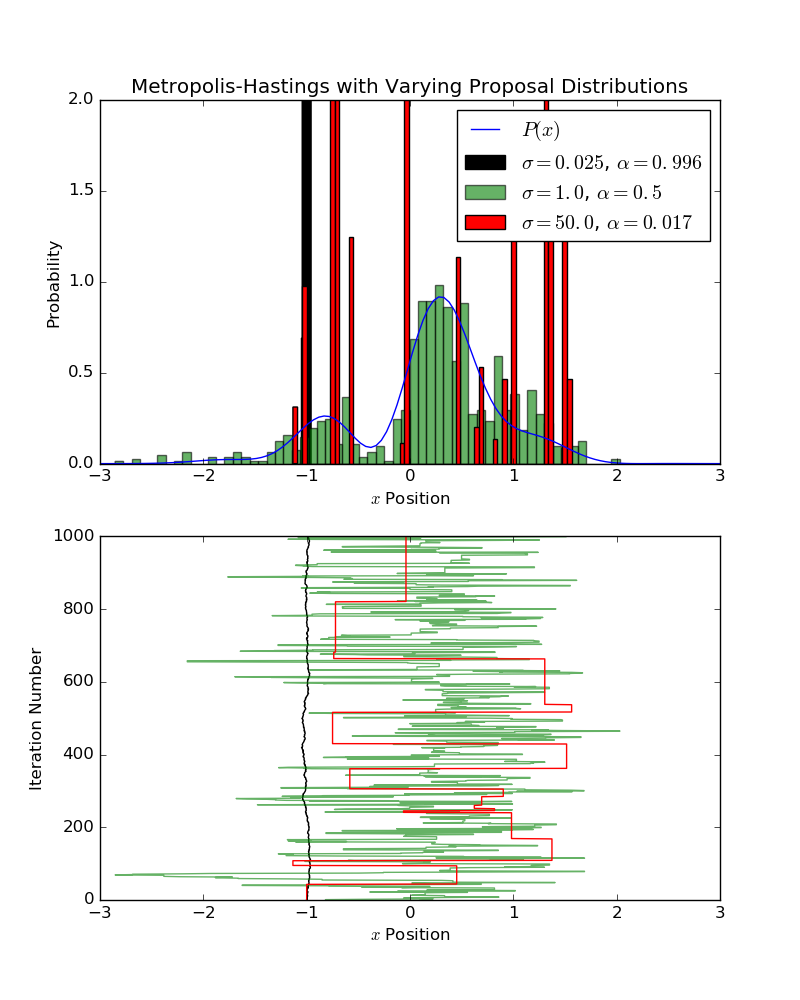
\includegraphics[width=\linewidth]{mcmc1.png}
  \caption{
    The Metropolis-Hastings algorithm was used to sample the probability space
    of equation \ref{eq:example} with a normal proposal distribution, run for
    $1\,000$ steps. The width of the proposal distribution was varied, where
    $\sigma$ is the standard deviation, and $\alpha$ is the acceptance rate. The
    top half shows the resulting probability distribution by taking the
    histogram of the random walk, as well as the true distribution $P(x)$. The
    bottom half shows the Markov chain and the position of each walker over
    time.
  }
  \label{fig:mcmc1}
\end{figure}

The program used in figure \ref{fig:mcmc1} was only run for $1000$ steps, and
the law of large numbers states that the random walk should approach the correct
distribution given a large number of steps. To test this, we ran the same
program again with $50\,000$ steps, shown in figure \ref{fig:mcmc2}. As
predicted, the results for the very narrow and very wide proposal distributions
improved over time. However, it should be noted that with a very small $\sigma$,
the walker was only able to explore the area around the local maxima where it
started. The walker with very large $\sigma$ still has a very low acceptance
rate, and the result is oversampling the global maxima. On the other hand, the
reasonably chosen $\sigma$ has a very good fit under the curve, which has only
improved over time.

\begin{figure}
  \centering
  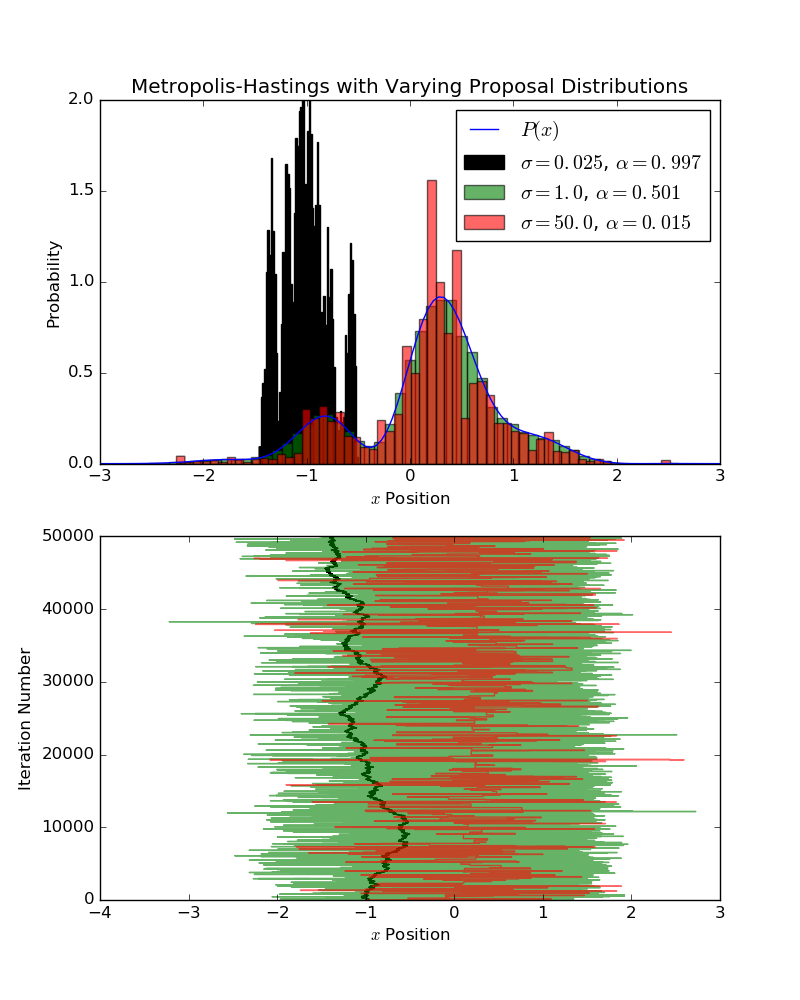
\includegraphics[width=\linewidth]{mcmc2.png}
  \caption{
    The Metropolis-Hastings algorithm was used in the same way as in figure
    \ref{fig:mcmc1} but with $50\,000$ steps. No other parameters were changed.
  }
  \label{fig:mcmc2}
\end{figure}

\subsubsection{The Burn-in Phase}
The burn-in phase refers to the process of the walkers moving toward an
equilibrium. The number of steps this takes is highly dependent on the choice of
starting values and how suitable the proposal distribution is. This time, all
parameters will be kept the same, so the walkers all start at $x_0 = -3$,
$\sigma = 0.2$, and are all run for $1\,000$ steps. The difference between the
two experiments is only the distribution done at the end, where in figure
\ref{fig:burn1} all steps are kept as the control case and \ref{fig:burn2} is
the experiment with burn-in, and the first $200$ steps are discarded.

\begin{figure}
  \centering
  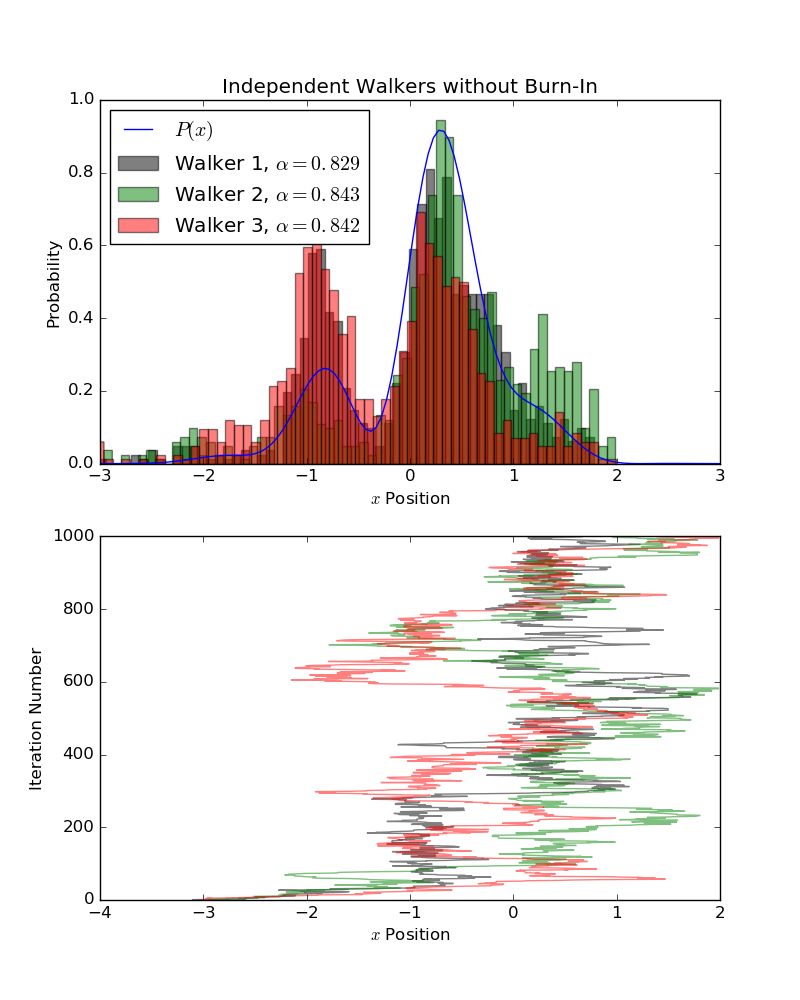
\includegraphics[width=\linewidth]{burn1.png}
  \caption{
    The Metropolis-Hastings random-walk for three identitcal walkers, starting
    at $x_0 = -3$, standard deviation $\sigma = 0.2$, and run for $1\,000$
    steps. This is the control case where all steps are kept. This is to compare
    with figure \ref{fig:burn2} where the burn-in phase is considered.
  }
  \label{fig:burn1}
\end{figure}

\begin{figure}
  \centering
  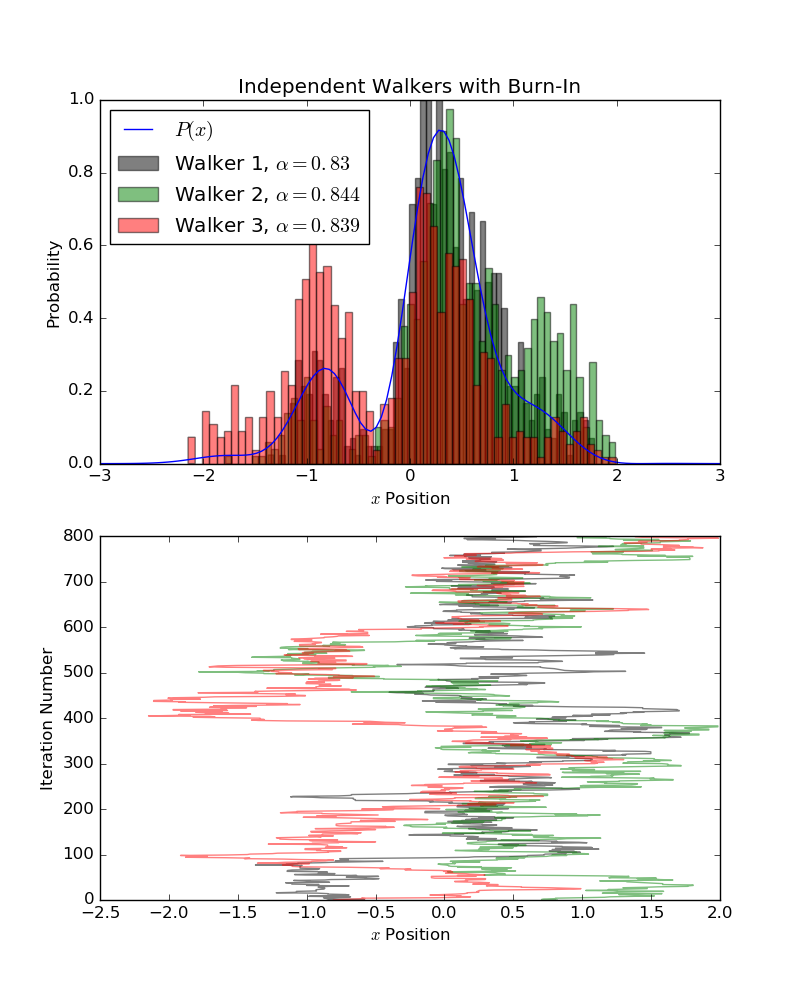
\includegraphics[width=\linewidth]{burn2.png}
  \caption{
    The Metropolis-Hastings random-walk with burn-in phase considered. The first
    $200$ of $1\,000$ steps were discarded. Since this was run with identical
    conditions as it was in figure \ref{fig:burn1}, the walks are very similar
    since the same seed was used. The only difference is which steps were
    discarded or kept.
  }
  \label{fig:burn2}
\end{figure}

By comparing figure \ref{fig:burn1} with figure \ref{fig:burn2}, the most
obvious difference is how the experiment that considers the burn-in phase can
avoid oversampling the local maxima centered around $x = -1$. The reason the
oversampling occurs in the first place is the walkers began at the edge of the
distribution, far away from the center of the distribution. This is not always a
problem very easily solved, and is improved by allowing the system to reach a
state closer to equilibrium before we begin considering every step.

